\chapter{Mapeamento de Código Limpo em Métricas de Código-fonte}
\label{chap:mapeamento}	

	Após a discussão teórica realizada na primeira parte dessa 	monografia, apresentaremos um mapeamento dos conceitos de código limpo em métricas de código-fonte. Nesse mapeamento usamos um conjunto de métricas para automatizar a busca por características do código-fonte. Em seguida, criamos uma interpretação dos valores das métricas, fazendo associações entre eles e as técnicas e conceitos relacionados a limpeza do código. Nosso objetivo é facilitar a detecção de trechos que poderiam sofrer alterações que os tornem mais expressivos, simples e flexíveis.


\section{Métricas de Código-fonte}

	Métricas são mecanismos automatizáveis para detecção de características obtidas através da análise do código-fonte.
	
	Existem várias abordagens diferentes para o uso de métricas. Em muitas pesquisas elas são usadas como mecanismos que permitem encontrar características nos códigos-fonte. Essas características serão usadas, por exemplo, na avaliação da qualidade do software \citep{meirelles:sbqs09}, ou para serem relacionadas com atributos dos projetos de software livre \citep{meirelles2010}. 
	
	No contexto de métodos ágeis, as métricas são importantes parâmetros para \textit{tracking} de projetos (acompanhamento do desenvolvimento do projeto). Por exemplo, contando linhas de código já produzidas, ou no cálculo da cobertura de teste.	Além disso, elas estão presentes na abordagem do modelo GQM (Goal, Question, Metrics), que é utilizado para gestão de projetos através da formulação de objetivos e questões que auxiliam na interpretação dos valores das métricas escolhidas.
	
	Nessa monografia usamos uma abordagem baseada na determinação de um conjunto de métricas que seja facilmente interpretado e que visa encontrar trechos de código que precisem de melhorias quanto a sua limpeza.
	
	Sabemos que existem muitas métricas e que quanto maior a quantidade delas calculada, mais difícil compreender os seus valores. Essa dificuldade é suficientemente grande para motivar a criação de ferramentas que automatizam a interpretação dos resultados obtidos. Uma dessas ferramentas é a Kalibro, descrita no artigo (\citep{meirelles:sbes09}). A mesma permite que o usuário configure intervalos numéricos que possibilitam uma interpretação qualitativa do valor de cada métrica. Assim, podemos usar intervalos como ``Bom'', ``Regular'' e ``Ruim'' ao invés de usar ``0 a 1/3'', ``1/3 a 2/3'' e ``2/3 a 1'', facilitando o entendimento e a classificação dos aspéctos medidos a partir do código-fonte.
	
	No entanto, ao considerar o uso de uma ferramenta como a Kalibro nesse trabalho, encontramos algumas dificuldades. Uma é a dependência da combinação de métricas para encontrar as características que procuramos, uma vez que há apenas suporte na Kalibro para interpretação de cada valor separadamente e não para conjuntos deles. Outro problema consiste em como definir os intervalos numéricos. Por exemplo, podemos usar os conceitos apresentados por Robert Martin \citep{Martin2008} para definir essas referências, porém, temos que considerar que diferentes linguagens e domínios de aplicação precisam de padrões de implementação distintos, como comenta Kent Beck \citep{Beck2007}.	
	
	Para evitar esses problemas selecionamos um subconjunto pequeno de métricas que espelha bem as características de código limpo procuradas. A seleção feita não é a única capaz de suprir os mesmos objetivos, pois outras combinações podem ser propostas e obter resultados semelhantes.
		
	Na formação desse subconjunto, a minimalidade não foi uma restrição. Optamos por não eliminar todas as métricas correlacinadas, pois em alguns casos, mesmo que elas indiquem coisas parecidas, elas nos fornecem alguns outros dados bastante relevantes.
	
	Dado a dificuldade em fixar valores para a interpretação das métricas, o mapeamento desenvolvido nessa pesquisa não tem como objetivo afirmar se um código é limpo ou não. Nossa proposta é formar um conjunto de métricas cujos valores expressem diferentes cenários relacionados com melhorias quanto a limpeza do código.
	
	
\section{O Mapeamento}

	O mapeamento proposto nesse trabalho visa facilitar a procura por problemas quanto a limpeza do código. A ideia é criar cenários que relacionem os conceitos de código limpo com métricas de código-fonte. Cada cenário é descrito através dos seguintes componentes:
	
\begin{itemize}
	\item Referências: conceitos de limpeza de código que motivaram a criação do cenário.
	\item Características: indicam a presença de falhas em relação as referências apresentadas.
	\item Métricas: mecanismos que permitem analisar o código a procura das características do cenário.
	\item Objetivo: quais devem ser as ideias principais durante a refatoração para eliminar o problema.
	\item Resultados Esperados: quais características devem ser encontradas no código quando terminar a refatoração para eliminação do cenário.
\end{itemize}	

	
	Quando algum cenário é detectado, sugerimos que o usuário analise o trecho indicado verificando se é possível refatorar o código para melhorar sua limpeza. Esse mapeamento não visa afirmar se existem problemas no código, mas sim indicar partes dele que talvez possam ser melhoradas de acordo com os importantes conceitos discutidos nessa trabalho.

	Para incentivar a avaliação de códigos ao longo de seu desenvolvimento, é muito importante que sua interpretação seja simples. Esperamos que a preocupação com a limpeza do código não emerja apenas quando ele estiver pronto, pois nessa fase é provável que ele tenha vários problemas e que seja muito complicado alterá-lo. Por esse motivo, montamos aguns cenários e escolhemos um conjunto pequeno de métricas que nos permite detectar as características procuradas.
	
	Infelizmente, não é possível mapear todos os conceitos de código limpo usando métricas. Por exemplo, não consguimos encontrar problemas relacionados a nomes pouco expressivos usando apenas métricas. Nesse caso, não é suficiente analisarmos somente a estrutura do código, precisaríamos entender o contexto em que cada nome é usado, e para isso, também seria necessária uma análise semântica.

	Existem dois tipos de métricas de código-fonte. Algumas avaliam características de métodos, outras de classes. As métricas do segundo tipo são normalmente somas ou médias dos valores das avaliadoras de métodos. Essa divisão de alvo do análise das métricas também existe no contexto dos cenários.


\subsection{Conjunto de Métricas}

	Abaixo apresentamos o conjunto selecionado de métricas.

\subsubsection{NC: Número de Chamadas}
                             
	A métrica NC calcula o número de métodos e atributos internos e externos usados por um método. Elementos exeternos são aqueles que pertencem a classes não relacionadas hierarquicamente com a classe da operação analisada. Os internos são os pertencentes a mesma classe. NC é uma contração para \textit{Number of Calls}.

	O valor dessa métrica pode variar entre zero e a soma do número de atributos e métodos presentes no sistema. Obtemos zero quando o método em análise não acessa nenhum atributo e não faz chamadas a métodos.
	

\subsubsection{NEC: Número de Chamadas Externas}

	A métrica NEC calcula o número de métodos e atributos externos acessados por um método. Definimos como externos os elementos pertencentes a classes não relacionadas hierarquicamente com a classe do método em análise. NEC é uma contração para \textit{Number of External Calls}.
	                                               
	NEC é uma adaptação da métrica ATFD (\textit{Access To Foreing Data} \citep{Marinescu02}) que calcula o número de atributos de classas não relacionadas que são acessados diretamente ou através de chamadas a métodos de acesso. 
	
	Seu valor pode variar de zero até o número total de métodos e atributos do sistema. Nesse caso, zero indica que não há comunicação entre o método e qualquer outra classe sem relação com a sua.
	
                          

\subsubsection{ECR: Taxa de Chamadas Externas}
                                         
	A métrica ECR calcula a taxa de chamadas externas realizadas por um método. Para isso, são necessários o número de chamadas externas (NEC) e o total de chamadas (NC) realizadas pelo método. O valor da taxa será o resultado da divisão de NEC por NC. ECR é uma contração para \textit{External Calls Rate}.
	
	Essa métrica é uma adaptação da LAA (\textit{Locality of Attribute Accesses} \citep{Lanza06}) que calcula o número de atributos pertencentes a mesma classe que o método em análise, dividido pelo número total de variáveis acessadas (incluindo atributos usados através de métodos de acesso). 
	
	Seu valor varia entre zero e um. Obtemos zero quando o método não possui chamadas externas e um quando todas as chamadas realizadas são externas.
	
	
	
\subsubsection{NCC: Número de Classes Chamadas}              
                                                                 
   	A métrica NCC calcula o número de classes das quais métodos são chamados ou atributos são acessados por um método. Nesse calculo não contamos classes que tenham relação hierarquica  com a classe do método em análise. NCC é uma contração para \textit{Number of Classes Called}.

	Essa métrica é uma adaptação da FDP (\textit{Foreign Data Providers} \citep{Lanza06}) que calcula o número de classes das quais atributos são acessados. Seu valor varia entre zero e o número total de classes do sistema. Obtemos zero quando o método não utiliza elementos de outras classes.

	
	
\subsubsection{NRA: Número de Atributos Alcançáveis}
                                           
	A métrica NRA calcula o número de atributos alcançáveis a partir de um método. Um atributo pode ser alcançado direta ou indiretamente. O acesso é direto quando o atributo é usado no próprio corpo do método, e é indireto quando existe uma chamada para algum método que usa o atributo direta ou indiretamente. NRA é uma contração para \textit{Number of Reachable Attributes}.
	          
	Para descobrirmos quantos atributos são alcançáveis por um método, podemos criar um grafo com atributos e métodos como vértices e os acessos e chamadas a eles como arestas. Com esse grafo criado, podemos encontrar os vértices atingíveis a partir do vértice que representa o método em análise. Então, contamos quantos deles são atributos. E assim, obtemos o número de atributos alcançáveis pelo método.
                                                           
	O valor dessa métrica varia entre zero e o total de atributos da classe do método. Obtemos zero quando o método não alcança nenhum atributo de sua classe e o valor máximo quando ele usa direta ou indiretamente todos os atributos de sua classe.
                          


\subsubsection{MaxNesting: Nível Máximo de Estruturas Encadeadas}
                         
	A métrica MaxNesting (\citep{Lanza06}) calcula o nível máximo de estruturas encadeados presentes no corpo de um método. MaxNesting é uma contração para \textit{Maximum Nesting Level}
	
	Seu valor varia entre zero e a quantidade total de quebras de fluxo do método. Obtemos zero quando o método não possui controladores de fluxo. Atingimos o valor máximo quando todas as quebras condicionais presentes no método encontran-se em níveis diferentes da mesma estrutura.
	
	Os comandos \textit{if}, \textit{while} e \textit{for} são alguns exemplos de controladores de fluxo bastante usados em diversas linguagens diferentes.                
	
                                                             

\subsubsection{CYCLO: Complexidade Ciclimática}

	A métrica CYCLO \citep{McCabe76} calcula o número de caminhos linearmente independentes no método analisado, conhecido como complexidade ciclomática. CYCLO é uma contração para \textit{Cyclomatic Complexity}.
	
	Seu valor varia de um até infinito. Obtemos um quando não há quebra do fluxo principal. Cada estrutura de controle de fluxo presente no corpo do método adiciona um no valor total da CYCLO.
	                          
	Quando os valores de MaxNesting e CYCLO são próximos, sabemos que muitos dos controladores de fluxo presentes no método estão encadeados em uma mesma estrutura. Quando são muito distantes, podemos concluir que os controladores estão espalhados em estruturas diferentes e que elas não são muito profundas.



\subsubsection{NP: Número de Parâmetros}

	A métrica NP calcula o número de parâmetros de um método. Seu valor pode variar de zero a infinito. Obtemos zero quando o método avaliado não possui parâmetros.

                                                             

\subsubsection{NRP: Número de Repasses de Parâmetros}

	A métrica NRP calcula o número de parâmetros recebidos pelo método em análise e repassados como argumento em chamadas a outras operações pertencentes a sua classe.                                                    
	
	Seu valor varia entre zero e o número de parâmetros do método (indicado pela métrica NP). Obtemos zero quando nenhum parâmetro é repassado. O valor máximo é atingido quando todos os parâmetros são usados como argumentos em alguma chamda de operção realizada no corpo do método. 
                                                      
                                                             

\subsubsection{LOC: Número de Linhas}

	A métrica LOC \citep{LK94} calcula o número de linhas efetivas de um método. Linhas compostas apenas por comentários ou vazias não são consideradas efetivas. LOC é uma contração para \textit{Lines of Code}.



\subsubsection{NOA: Número de Atributos}

	A métrica NOA calcula o número de atributos de uma classe. Seu valor varia entre zero e infinito. Obtemos zero quando a classe analisada não possui atributos. NOA é uma contração para \textit{Number of Attributes}.
                          


\subsubsection{NOM: Número de Métodos}

	A métrica NOM calcula o número de métodos de uma classe. Seu valor varia entre zero e infinito. Obtemos zero quando a classe não possui métodos. NOM é uma contração para \textit{Number of Methods}.
                                                            
         

\subsubsection{Média de NEC: Média do Número de Chamadas Externas}
         
	Média de NEC calcula a média do número de chamadas de métodos e acessos a atributos externos a classe analisada por método.


\subsubsection{Média de NP: Média do Número de Parâmetros}

	Média de NP calcula a média do número de parâmetros por método da classe analisada.
	   


\subsubsection{Média de NRP: Média do Número de Repasses de Parâmetros}        

	Média de NRP calcula a média do número de repasses de parâmetros por método da classe analisada.


                                                        
\subsubsection{SLOC: Soma do Número de linhas}
                                          
	A métrica SLOC calcula a soma do número de linhas efetivas de todos os métodos de uma classe. Ou seja, seu resultado é a soma dos valores do LOC de cada método da classe.



\subsubsection{AMLOC: Média do Número de Linhas Por Método}
                                   
	AMLOC calcula a média do número de linhas efetivas por método da classe analisada.
	


\subsubsection{LCOM4: Falta de Coesão Entre Métodos}
    
	A métrica LCOM4 \citep{HM96} calcula a falta de coesão da classe analisada. Para isso, montamos um grafo cujos vértices são os atributos e métodos da classe. Cada aresta desse grafo representa o acesso de um atributo ou a chamada de método através de um outro método. Quando o grafo estiver pronto, contamos quantas componentes conexas existem nele. Esse número indica a quantidade de subconjuntos em que a classe está dividida. LCOM4 é uma forma compacta para 
	
	O seu valor varia entre um e infinito. Obtemos um quando a classe não possui subdivisões. Ou seja, quando a classe é bastante coesa. Normalmente, desejamos classes que não possuem conjuntos isolados de métodos e atributos, pois o número de subdivisões costuma indicar a quantidade de classes que deveriam existir para que cada uma fosse responsável por apenas um contexto.
	     

	  

\subsection{Os Cenários}

\subsubsection{Método Grande}
	
	O que motivou a formação desse cenário foi o conceito de composição de métodos, a necessidade de evitar estruturas encadeadas e a possibilidade de usar cláusula guarda.
	
	Métodos grandes tem como principal característica um elevado número de linhas. Verificamos que o método possui muitas linhas quando o valor da métrica LOC está alto. Outras características desse cenário são o elevado número de quebras condicionais de fluxo, indicada por um valor alto da CYCLO, e profundas estruturas com condicionais encadeados, indicada por um valor alto do MaxNesting. 
	
	Durante a refatoração desse cenário, nosso objetivo é diminuir o número de linhas (reduzir o LOC), diminuir a complexidade ciclomática (reduzir o CYCLO) e eliminar as estruturas encadeadas (reduzir o MaxNesting) no método em análise. Conseguimos atingir esses obejetivos decompondo o método grande em métodos menores. Normalmente começamos essa decomposição passando os blocos de código dos desvios de fluxo para outros lugares, pois esses são conjuntos de operações evidentemente isoladas do resto do método.
	
	Após a refatoração de todas as ocorrências desse cenário na classe em análise, esperamos que a sua média de linhas por método (média de LOC) e as profundidades máximas de estruturas encadeadas de cada método (o MaxNesting) abaixem. Provavelmente a complexidade ciclomática da classe (CYCLO) não sofrerá alterações. Isso acontece porque normalmente espalhamos essas quebras de fluxo em outros métodos da mesma classe, mas não as eliminamos da sua lógica. Teremos uma redução da complexidade ciclomática, quando parte do código for eliminado, ou trasferido para métodos de outras classes. Além disso, pode acontecer um aumento no número de métodos da classe, um aumento do número de métodos de outras classes ou até a criação de novas classes.
	
	Possuir muitas funcionalidades e parâmetros são mais duas características desse cenário. Porém, não precisamos nos preocupar com elas diretamente. Suas quantidades serão reduzidas como consequência da refatoração baseada nos outros aspéctos citados.

   	Para exemplificar esse cenário, vamos analisar o método \textit{custosAPartirDoVertice(vertice)} (\ref{metodo_grande}). Nessa avaliação, devemos calcular os valores das métricas que indicam a presença das características do problema descrito. 
    
\lstinputlisting[label=metodo_grande, caption={O método custosAPartirDoVertice é um exemplo de método grande}]{codigos/exemplos_para_os_cenarios/metodo_grande}                                      
          
	Quando contamos o número de linhas efetivas desse método, obtemos \textit{LOC = 17}. Ao contabilizar a quantidade de controladores de fluxo, chegamos a \textit{CYCLO = 6}. E para finalizar, temos que a profundidade máxima entre as estruturas de controladores encadeados, medida por MaxNesting, é igual a 4. 
	
	Como consideramos todos os valores adquiridos nessa análise altos para esse método, podemos dizer que encontramos nele todas as características de um método grande. Então, concluímos que ele está presente nesse cenário. Com base nessa informação, devemos refatorar esse código para que ele deixe de ser um método grande e melhore a sua limpeza.
	
	
\subsubsection{Método com Muitos Fluxos Condicionais}

	As referências que motivaram a criação desse cenário são a composição de métodos e o uso de exceções.
	
	Esse cenário acontece quando temos métodos que são complexos mas não necessariamente grandes. Sua principal característica é possuir muitas quebras condicionais de fluxo (valor alto da CYCLO). Também é comum encontrarmos longas estruturas com condicionais encadeados (valor alto de MaxNesting).
	
	Durante a refatoração desse cenário, buscamos minimizar a complexidade ciclomática (CYCLO) e a profundidade máxima de estruturas encadeadas (MaxNesting) do método, pois queremos deixar o código mais simples e direto. Podemos nos basear na decomposição de métodos para atingirmos nossos objetivos.
	
	Depois das modificações, esperamos que o a profundidade máxima de estruturas encadeadas tenha diminuído (redução do MaxNesting). Quando a refatoração for baseada no uso de exceções, como \textit{try catch} é provável que a complexidade ciclomática do método não se altere, pois essas estruturas também são contadas como desvios de fluxo no calculo da CYCLO. Pode acontecer também um aumento no número de métodos da classe, porque, em alguns casos, o conteúdo do bloco de cada desvio condicional é deslocado para novos métodos. 
           
	Para exemplificar esse cenário, usaremos o método \textit{deletaPaginasETodasAsReferencias} (\ref{metodo_com_muitos_fluxos_condicionais}). Quando analisamos esse bloco de código usando as métricas indicadas nesse cenário, encontramos os valores \textit{CYCLO} = 4 e \textit{MaxNesting} = 3. Ambos são valores considerados altos para esse método. Ou seja, temos muitos controladores de fluxo e uma longa estrutura desses controladores encadeados. Como encontramos todas as características desse cenário nesse exemplo, podemos dizer que esse método tem muitos fluxos condicionais. 
	
\lstinputlisting[label=metodo_com_muitos_fluxos_condicionais, caption={O método deletaPaginasETodasAsReferencias é um exemplo de método com muitos fluxos condicionais}]{codigos/exemplos_para_os_cenarios/metodo_com_muitos_fluxos_condicionais}               

	Analisando o código a procura de possíveis refatorações, observamos que esse método realiza três operações e a verificação de falha para cada uma delas. Esse tratamento de erros poderia ser feito usando \textit{try catch}. Essa mudança diminuiria o valor de \textit{MaxNesting} e de \textit{CYCLO}, reduzindo bastante o problema encontrado. O resultado dessa refatoração é o método exposto em \ref{uso_de_try_catch_no_problema_com_fluxos_condicionais}.
                                                         
\lstinputlisting[label=uso_de_try_catch_no_problema_com_fluxos_condicionais, caption={Uma refatoração usando \textit{try catch} para o método deletaPaginasETodasAsReferencias}]{codigos/exemplos_para_os_cenarios/uso_de_try_catch_no_problema_com_fluxos_condicionais}

	Com essa refatoração deixamos o método mais simples e fora desse cenário.


\subsubsection{Método com Muitos Parâmetros}

	Esse é um cenário bastante simples. Sua referência base é o agrupamento de parâmetros em objetos. A principal característica de um método que está nesse contexto é ter um elevado número de parâmetros (valor alto de NP).
	
	Durante a refatoração desse cenário, o objetivo é minimizar o número de parâmetros recebidos (diminuir o NP). Os resultados esperados após a refatoração são a redução do número de parâmetros (redução do NP) e o aumento do número de classe. Esse aumento ocorre quando criamos classes para agrupar os parâmetros que pertencem a um mesmo contexto em um único objeto.
	                                       
	Para exemplificar esse cenário, usaremos o método \textit{calculaQuantidadeDeDias} (\ref{metodo_com_muitos_parametros}). Quando calculamos sua quantidade de parâmetros, obtemos \textit{NP = 6}. Como consideramos esse valor alto para a métrica NP, podemos dizer que esse método está no contexto de método com muitos parâmetros.                    

\lstinputlisting[label=metodo_com_muitos_parametros, caption={O método calculaQuantidadeDeDias é um exemplo de método com muitos parametros}]{codigos/exemplos_para_os_cenarios/metodo_com_muitos_parametros}                   
                                
	Ao analisarmos os parâmetros presentes nesse exemplo, podemos notar que eles representam duas datas formadas por \textit{dia, mês e ano}, que indicam o início e o fim de um período. Então, uma refatoração possível para esse código seria criar uma classe \textit{Data} da qual cada objeto representasse uma dessas datas. Assim, reduziríamos o valor de \textit{NP} de seis para dois, eliminando o problema de alto número de parâmetros desse método (\ref{refatoracao_para_metodo_com_muitos_parametros}). 

\lstinputlisting[label=refatoracao_para_metodo_com_muitos_parametros, caption={O método calculaQuantidadeDeDias depois da refatoração para redução do número de parâmetros}]{codigos/exemplos_para_os_cenarios/refatoracao_para_metodo_com_muitos_parametros}          

\subsubsection{Muita Passagem de Parâmetros Pela Classe}
	
	Esse é o primeiro cenário que descrevemos relacionado com a avaliação da classe como um todo e não de métodos separados. Suas referências são o agrupamento de parâmetros em objetos e a transformação de parâmetros em variáveis de instância.
	
	Podemos separar esse cenário em dois casos diferentes. O primeiro caso trata do repasse de muitos parâmetros. Sua característica é ter uma elevada média de parâmetros repassados (alta média de NRP). Parâmetros repassados são aqueles recebidos por um método que os repassam em chamadas a operações. O segundo caso se preocupa com a elevada média do número de parâmetros por método da classe analisada (alta média de NP).       
		     
	Então, é comum que os métodos de classes com muita passagem de parâmetro tenham muitos ou repassem muitos parâmetros ou recebam variáveis que são usadas apenas em chamadas a outros métodos.	O método \textit{acumulaRelatorioDasMetricasGlobais} (\ref{metodo_com_muito_repasse_de_parametros}) exemplifica a existência de parâmetros que são apenas repassados em chamadas a outras operações.
	                                                               
\lstinputlisting[label=metodo_com_muito_repasse_de_parametros, caption={O método custosAPartirDoVertice é um exemplo de método com muito repasse de parâmetros}]{codigos/exemplos_para_os_cenarios/metodo_com_muito_repasse_de_parametros}                                     
	
	Os objetivos durante a refatoração são diminuir o número de repasses de parâmetros pela classe (diminuir o NRP) e reduzir o número de parâmetros dos métodos (reduzir o NP). Fazemos isso tranformando os parâmetros muito repassados ou usados em muitos métodos, em atributos e criando objetos para guardar conjuntos de parâmetros relacionados.
	
	Os resultados esperados após a refatoração do código são a redução da média do número de parâmetros por método (redução da média de NP) e do número de repassagem de parâmetro (redução do NP), e o aumento do número de variáveis de instância. Além disso, pode ocorrer um aumento no número de classes, caso aconteça a junção de variáveis em um único objeto.	           


\subsubsection{Método ``Invejoso''}
	
	Método ``invejoso'' é aquele que usa um elevado número de métodos e atributos de poucas classes não relacionadas hierarquicamente com a sua própria. Mapeando essas características em métricas de código-fonte, temos nesse cenário alta ECR, que indica a taxa de chamadas a métodos e atributos externos, e baixa NCC, que representa o número de classes não relacionadas chamadas pelo método.
	
	A preocupação durante uma refatoração nesse contexto, deve ser a minimização do número de chamadas externas, calculado através do NEC. A principal referência desse cenário é a delegação de tarefa.
	
	Após a refatoração, esperamos uma redução do número de chamadas externas (diminuição do NEC), da taxa de chamadas externas (diminuição do ECR) e da média do número de chamadas externas da classe (diminuição da média de NEC).
                      
	Para exemplificar esse cenário, usaremos o método \textit{salarioDoMes} da classe \textit{CalculaReceita} (\ref{metodo_invejoso}). Quando calculados a taxa de chamadas externas feitas por esse método, obtemos \textit{ECR = NEC/NC = 4/4 = 1}. O resultado é o valor máximo para essa métrica, o que indica que o método possui apenas chamadas externas e que, portanto, tem alto acoplamento. Devemos, então, calcular a quantidade de classes diferentes que são chamadas por esse método. O resultado é \textit{NCC = 1}. Esse valor indica que todos os elementos externos usados são da mesma classe. Como a taxa de chamadas externas é alta e todos os elementos externos usados são da mesma classe, podemos dizer que o método \textit{salarioDoMes} está no cenário de método ``invejoso''.

	\lstinputlisting[label=metodo_invejoso, caption={Método salarioDoMes com problemas de ``inveja''}]{codigos/exemplos_para_os_cenarios/metodo_invejoso}                                      

	Para resolver esse problema, podemos passar para a classe empregado o método \textit{salarioDoMes} (\ref{refatoracao_para_metodo_invejoso}). Quando isso acontecer os valores das suas métricas serão \textit{ECR = NEC/NC = 0/4 = 0} e \textit{NCC = 0}, o que resolve o seu problema de ``inveja'' dada a redução do acoplamento entre as classes \textit{CalculaReceita} e \textit{Empregado}. 

	\lstinputlisting[label=refatoracao_para_metodo_invejoso, caption={Redução do acoplamento entre as classes CalculaReceita e Empregado}]{codigos/exemplos_para_os_cenarios/refatoracao_para_metodo_invejoso}


\subsubsection{Método Dispersamente Acoplado}
	
	Um método dispersamente acoplado utiliza um elevado número de atributos e métodos de várias classes não relacionadas hierarquicamente com a sua. Assim como no contexto de método ``invejoso'', nesse cenário temos um valor alto de ECR, indicando que o uso de métodos e atributos externos é maior do que de internos. Porém, a diferença entre eles é o número de classes não relacionadas chamadas pelo método, sendo o valor do NCC alto nesse cenário e baixo para métodos ``invejosos''.
	
	Durante a refatoração, devemos focar na redução do número de chamadas externas que é calculado através da métrica NEC. Esse cenário foi criado com base nas referências de objeto centralizador e objeto método.
	
	Os resultados esperados após a refatoração é a redução do número de chamadas externas e da média dela na classe do método analisado (NEC e média de NEC) e a diminuição do número de classes não relacionadas chamadas (NCC). É possível que ocorra um aumento no número de classes. Isso acontecerá quando uma classe for criada para centralizar o diálogo entre as classes não relacionadas, sendo sacrificado para que as outras possam manter suas características e serem reutilizadas em outros projetos. 
	  
	Para exemplificar esse cenário, usaremos o método \textit{adicionaDadosDaRodada}. Quando o avaliamos usando as métricas \textit{ECR} e \textit{NCC} obtemos valores elevados, pois nesse código são usados seis métodos externos de quatro classes diferentes. Com esses resultados dizemos que esse método é dispersamente acoplado.
  
\lstinputlisting[label=metodo_dispersamente_acoplado, caption={Método ``adicionaDadosDaRodada'' dispersamente acoplado}]{codigos/exemplos_para_os_cenarios/metodo_invejoso}                                      
  

\subsubsection{Classe Pouco Coesa}

	As referências desse cenário são a maximização da coesão e o princípio da responsabilidade única. Assim como o cenário que indica muita passagem de parâmetros pela classe, esse contexto analisa a classe como um todo.
	
	A principal característica de uma classe pouco coesa é possuir subdivisões em grupos de métodos e atributos que não se relacionam (valor de LCOM4 > 1), ou possuir métodos que alcançam em média poucos atributos da propria classe (média de NRA <<< NOA). Nessse contexto, dizemos que um método alcança um atributo se ele usa o atributo no seu próprio corpo ou de forma indireta, ou seja, através da chamada de algum método que usa o atributo direta ou indiretamente.
	   
	Na figura abaixo temos a representação abstrata de uma classe. Os círculos cinzas são os métodos e os azuis atributos da classe. As setas representam chamadas e acessos entre esses elementos. Quando contamos os grupos de elementos conexos, obtemos \textit{LCOM4 = 2}, e no cálculo do número médio de atributos atingidos por cada método, obtemos \textit{média de NRA = 1.16}. Como o valor de \textit{LCOM4} é alto e o de \textit{NRA} é muito menor do que o número total de atributos (\textit{NOA = 3}), podemos classificar essa classe como pouco coesa.
		
	\begin{figure}[htb]
		\centering
		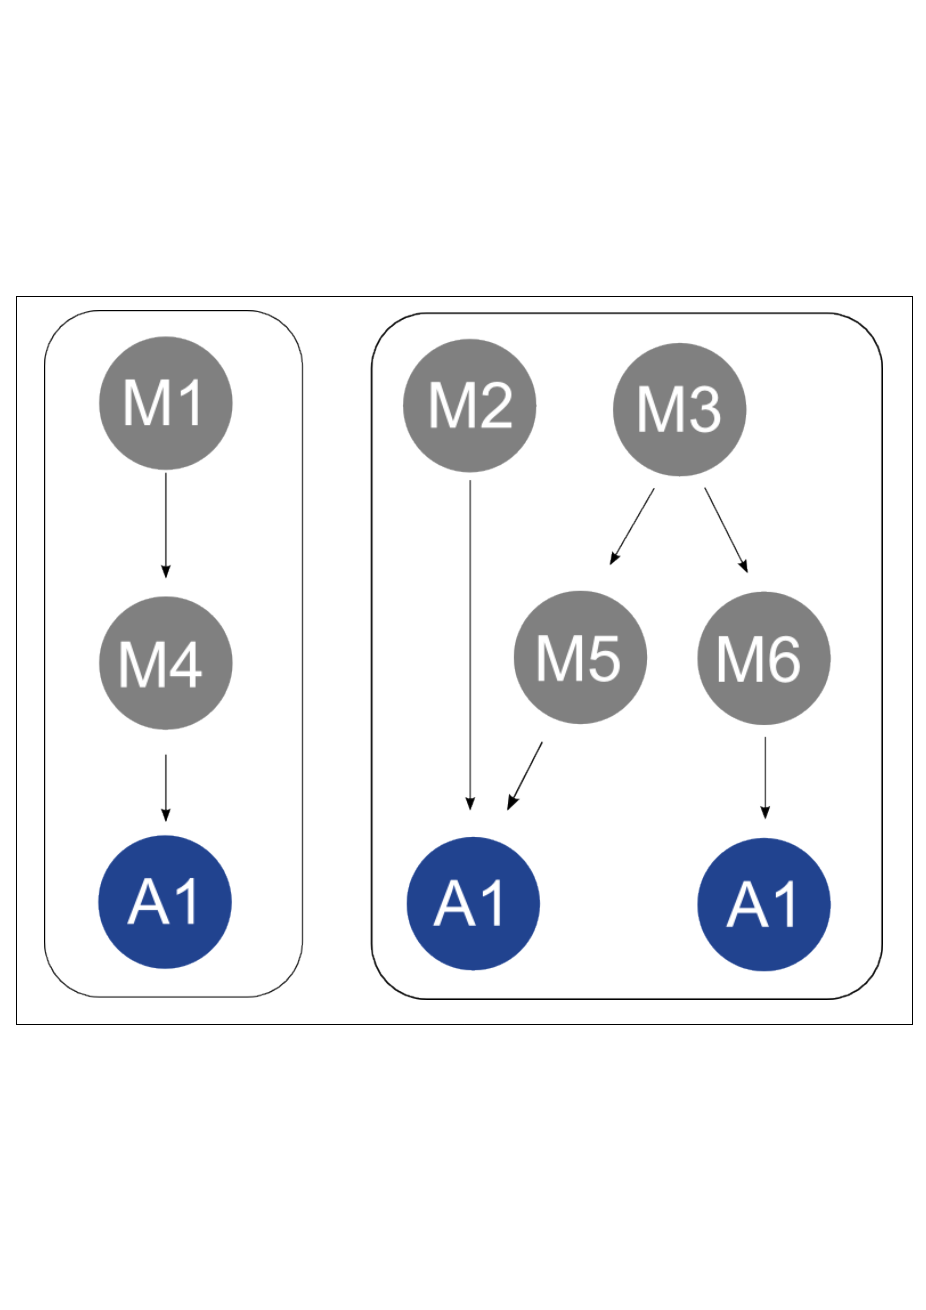
\includegraphics[trim = 0mm 50mm 0mm 60mm, clip, width=0.8\textwidth]{codigos/exemplos_para_os_cenarios/classe_pouco_coesa.png}
		\caption{Representação abstrata de uma classe pouco coesa}
		\label{classe_pouco_coesa}
	\end{figure}
	
	Os objeticos durante a refatoração são aumentar a coesão (diminuir a LCOM4) e diminuir a diferença entre média do número de atributos alcançáveis (NRA) e o número de atributos da classe analisada (NOA). Portando, uma boa refatoração para esse cenário seria separar as subdivisões já existentes na classe analisada em classes mais coesas.
	
	Como resultado da refatoração desse cenário, esperamos encontrar um aumento do número de classes. Além disso, desejamos que as classes existentes não tenham subdivisões (LCOM4 = 1) e que a média do número de atributos alcançáveis por cada método seja mais próxima da quantidade de atributos da classe (média de NRA próxima de NOA).
                  





